\newpage
\section{Sequences}

In this section we will precise the sequences of some use cases.

\subsection{Regular use of git commands}

\paragraph{}
When running regular git commands, the requests of the user pass through a SSH server. His SSH public key serves as an identifier. The SSH server will then forward the request to the authentication and authorization layer, that will forward the command to the git server if the user is authorized to do so. The figure \ref{fig:sequence_git} shows the sequence diagram of this use case.

\begin{figure}[h]
    \centering
    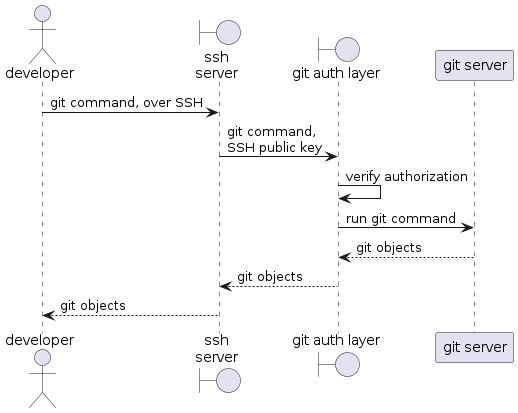
\includegraphics[width=0.7\textwidth]{iteration_02/diagrams/sequence_git.png}
    \caption{Sequence diagram of running a regular git command against the system}
    \label{fig:sequence_git}
\end{figure}

\subsection{LFS commands}

\paragraph{}
In the case of an LFS command, the user first need to get a POA. Then he can request some signed links, and only then upload or download objects. 

\paragraph{}
There is two types of implementation for the links. Either the storage is able to verify these links itself (such as MinIO, or AWS S3), so we can just generate these links and redirect the user to the storage itself; or it does not (such as a regular file system or a NAS), so we need to generate a proxy that will verify the links and then serve the files to the user. Another use of this second implementation would be to reduce the size of the exposed apis: all lfs-related requests would pass through the server, and we don't expose the storage directly to the user. The figure \ref{fig:sequence_lfs} shows the sequence diagram of this use case.


\begin{figure}[ht]
    \centering
    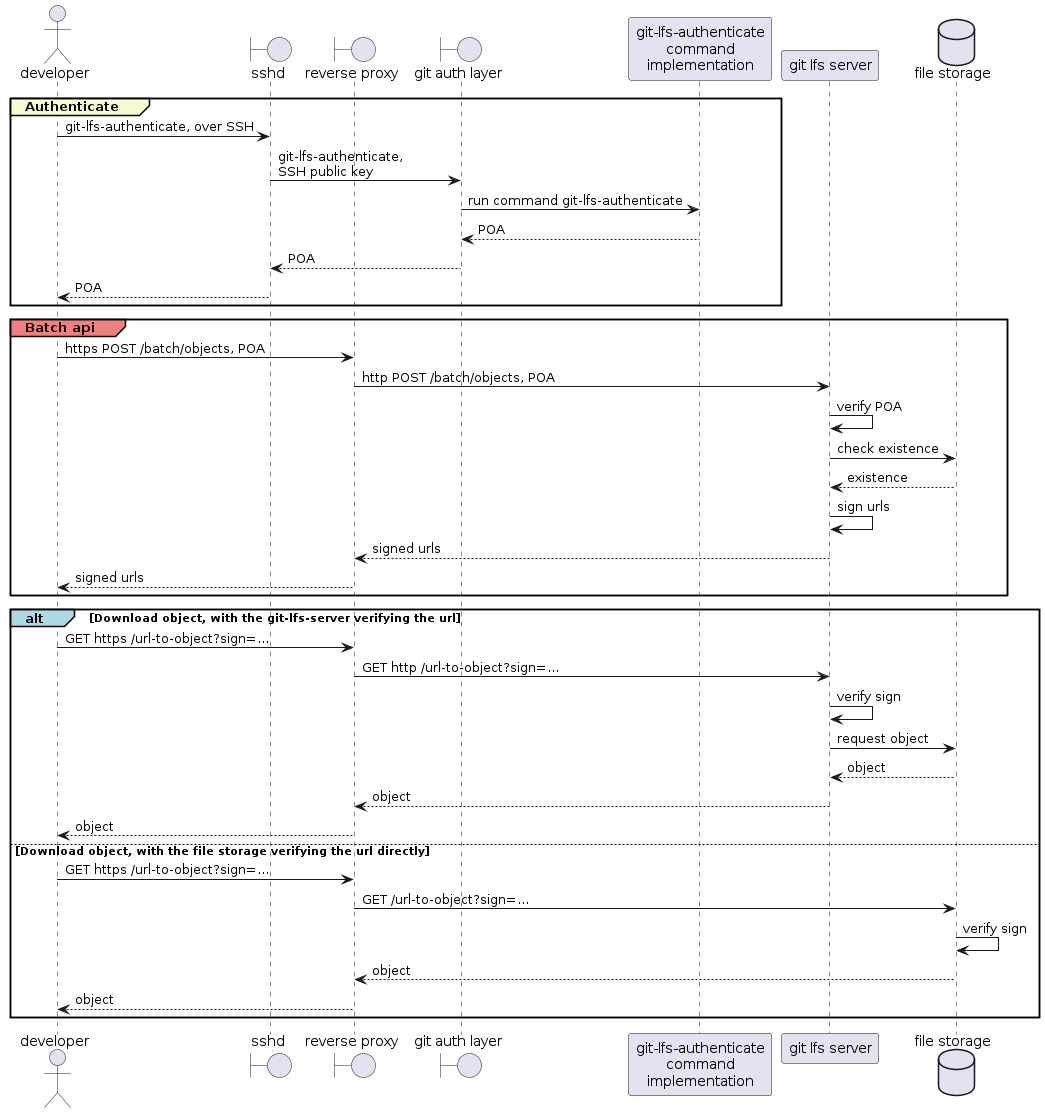
\includegraphics[width=1\textwidth]{iteration_02/diagrams/sequence_lfs.png}
    \caption{Sequence diagram of running lfs git command against the system}
    \label{fig:sequence_lfs}
\end{figure}
